\documentclass[12pt]{article}

%%%%%%%%%%%%%%%%%%%%%%%%%%%%%%%%%%%%%%%%%%%%%%%%%%%%%%%%%%%%%%%%%%%%%%%%%%%%%%%%%%%%%%%%%%%%%%%%%%%%
% Math
\usepackage{fancyhdr} 
\usepackage{amsfonts}
\usepackage{amsmath}
\usepackage{amssymb}
\usepackage{amsthm}
%\usepackage{dsfont}

%%%%%%%%%%%%%%%%%%%%%%%%%%%%%%%%%%%%%%%%%%%%%%%%%%%%%%%%%%%%%%%%%%%%%%%%%%%%%%%%%%%%%%%%%%%%%%%%%%%%
% Macros
\usepackage{calc}

%%%%%%%%%%%%%%%%%%%%%%%%%%%%%%%%%%%%%%%%%%%%%%%%%%%%%%%%%%%%%%%%%%%%%%%%%%%%%%%%%%%%%%%%%%%%%%%%%%%%
% Commands and Custom Variables	
\newcommand{\problem}[1]{\hspace{-4 ex} \large \textbf{Problem #1} }
%\let\oldemptyset\emptyset
%\let\emptyset\varnothing
\newcommand{\norm}[1]{\left\lVert#1\right\rVert}
\newcommand{\sint}{\text{s}\kern-5pt\int}
\newcommand{\powerset}{\mathcal{P}}
\renewenvironment{proof}{\hspace{-4 ex} \emph{Proof}:}{\qed}
\newcommand{\solution}{\textit{Solution}:\bigbreak}
\newcommand{\RR}{\mathbb{R}}
\newcommand{\NN}{\mathbb{N}}
\newcommand{\QQ}{\mathbb{Q}}
\newcommand{\ZZ}{\mathbb{Z}}
\newcommand{\CC}{\mathbb{C}}
\newcommand{\VV}{\mathbb{V}}
\newcommand{\FF}{\mathbb{F}}
\renewcommand{\Re}{\operatorname{Re}}
\renewcommand{\Im}{\operatorname{Im}}

\newcommand{\bigO}{\mathcal{O}}

\newcommand{\PP}{\mathcal{P}}

\renewcommand{\vec}[1]{\boldsymbol{\mathbf{#1}}}

\newcommand{\editnote}[1]{\textcolor{red}{\textbf{\MakeUppercase{#1}}}}


%%%%%%%%%%%%%%%%%%%%%%%%%%%%%%%%%%%%%%%%%%%%%%%%%%%%%%%%%%%%%%%%%%%%%%%%%%%%%%%%%%%%%%%%%%%%%%%%%%%%
%page
\usepackage[margin=1in]{geometry}
\usepackage{setspace}
%\doublespacing
\allowdisplaybreaks
\pagestyle{fancy}
\fancyhf{}
\rhead{Shaw \space \thepage}
\setlength\parindent{0pt}
\usepackage{color}

%%%%%%%%%%%%%%%%%%%%%%%%%%%%%%%%%%%%%%%%%%%%%%%%%%%%%%%%%%%%%%%%%%%%%%%%%%%%%%%%%%%%%%%%%%%%%%%%%%%%
%Code
\usepackage{listings}
\usepackage{courier}
\lstset{
	language=Python,
	showstringspaces=false,
	formfeed=newpage,
	tabsize=4,
	commentstyle=\itshape,
	basicstyle=\ttfamily,
}

%%%%%%%%%%%%%%%%%%%%%%%%%%%%%%%%%%%%%%%%%%%%%%%%%%%%%%%%%%%%%%%%%%%%%%%%%%%%%%%%%%%%%%%%%%%%%%%%%%%%
%Images
\usepackage{graphicx}
\graphicspath{ {images/} }
\usepackage{float}

%tikz
\usepackage[utf8]{inputenc}
%\usepackage{pgfplots}
%\usepgfplotslibrary{groupplots}

%%%%%%%%%%%%%%%%%%%%%%%%%%%%%%%%%%%%%%%%%%%%%%%%%%%%%%%%%%%%%%%%%%%%%%%%%%%%%%%%%%%%%%%%%%%%%%%%%%%%
%Hyperlinks
%\usepackage{hyperref}
%\hypersetup{
%	colorlinks=true,
%	linkcolor=blue,
%	filecolor=magenta,      
%	urlcolor=cyan,
%}

\begin{document}
	\thispagestyle{empty}
	
	\begin{flushright}
		Sage Shaw \\
		m503 - Fall 2018 \\
		\today
	\end{flushright}
	
\begin{center}{\large \textbf{Possible Exam 1}}\end{center}
\bigbreak

\hspace{-.5 ex}\problem{1} In $\PP_2(\RR)$ consider the standard monomial basis $b_1 = (1, x, x^2)$. Let $T: \PP_2(\RR) \to \PP_2(\RR)$ be differentiation. Write $M(T, b_1)$.

\bigbreak
\bigbreak
\bigbreak
\bigbreak
\bigbreak
\bigbreak
\bigbreak
\bigbreak
\bigbreak
\bigbreak
\bigbreak
\bigbreak
\bigbreak
\bigbreak
\bigbreak
\bigbreak
\bigbreak
\bigbreak
\bigbreak
\bigbreak

Consider the alternative basis $b_2 = (1, x, x^2-1)$. These are the first three Legendre Polynomials. They have nice properties and are used often in applied math. Write $M(T, b_2)$.


\pagebreak
%%%%%%%%%%%%%%%%%%%%%%%%%%%%%%%%%%%%%%%%%%%%%%%%%%%%%%%%%%%%%%%%%%%%%%%%%%%%%%%%%%%%%%%%%%%%%%%%%%%%
\problem{2} For the following propositions, decide if they are true or false, and cite a theorem you would use to prove so. If the proposition is nonsensical, explain why it is so.
\begin{enumerate}
	\item $\dim \RR^2 = \dim \CC^2$ \\ \\ \\ \\ \\ \\
	\item On the space of Polynomials: $\PP(\RR)$, let $I$ be the mapping $$I(\vec{p}(x)) = \int_{-\pi}^{\pi} (x^2-1)\vec{p}(x) dx\text{.}$$ Then $I(x^2-1)$ is a subspace of $\PP(\RR)$. \\ \\ \\ \\
	\item $ \dim \CC^2 = 4$ \\ \\ \\ \\ \\ \\
	%\item $\{(1,0), (0,1), (i,0), (0,i) \}$ is a basis for $\CC^2$ \\ \\ \\ \\ \\ \\
	\item Consider the vector space $V = \CC^2$ over the field $\RR$. Here vectors look like $(z_1, z_2)$ where $z_1$ and $z_2$ are complex numbers and scalars are real numbers. Then %$\dim V = 4$. \\ \\ \\ \\ \\ \\
	$\{(1,0), (0,1), (i,0), (0,i) \}$ is a basis for $V$.
\end{enumerate}

\pagebreak
%%%%%%%%%%%%%%%%%%%%%%%%%%%%%%%%%%%%%%%%%%%%%%%%%%%%%%%%%%%%%%%%%%%%%%%%%%%%%%%%%%%%%%%%%%%%%%%%%%%%
\problem{3} Let $V = \RR^2$ and let $U = \{(3y, y) \mid y \in \RR\}$. Consider the quotient space $V/U$. compute the following.
\begin{enumerate}
	\item $\dim V = $ \\
	\item $\dim U = $ \\
	\item $\dim V/U = $\\
\end{enumerate}
\bigbreak
Consider the element of the quotient space $(3,3) + U \in V/U$. Plot the subspace $U$, the element of the quotient space $(3,3) + U$ and the vector $(3,3) \in \RR^2$ in the same plane below. Be sure to label everything clearly for full credit.

\begin{figure}[H]
	%\caption{Equispaced points}
	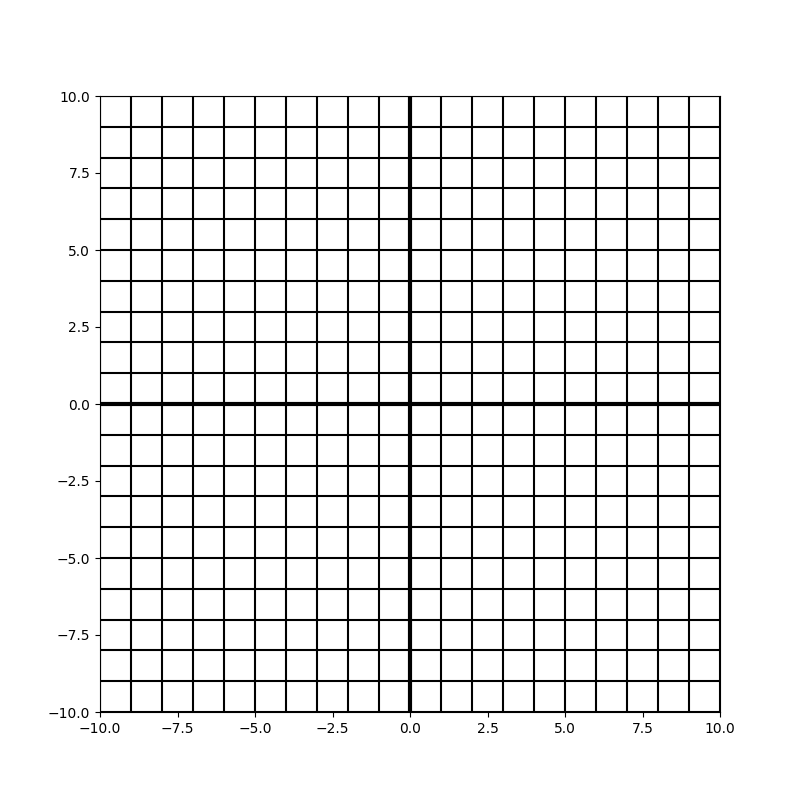
\includegraphics[width=.8\textwidth]{cartesian_grid}
	\centering
\end{figure}

\pagebreak
%%%%%%%%%%%%%%%%%%%%%%%%%%%%%%%%%%%%%%%%%%%%%%%%%%%%%%%%%%%%%%%%%%%%%%%%%%%%%%%%%%%%%%%%%%%%%%%%%%%%
\problem{4} Let $T: \RR \to \PP_3(\RR)$. If $T$ is linear, what are the possible dimensions of the null space and range?
\\ \\ \\ \\ \\ \\ \\ \\ \\ \\ \\ \\ \\ \\

Suppose that $T$ is surjective. Prove it is not linear.

\pagebreak
%%%%%%%%%%%%%%%%%%%%%%%%%%%%%%%%%%%%%%%%%%%%%%%%%%%%%%%%%%%%%%%%%%%%%%%%%%%%%%%%%%%%%%%%%%%%%%%%%%%%
\problem{5} What is the rank of the matrix $\begin{bmatrix}1 & 2 & 3 \\ 4 & 5 & 6 \\ 7 & 8 & 9 \end{bmatrix}$.


\end{document}
